\begin{name}
	{\tenchude}
	{\tendethi}
	{\tentruong}
	{\thoigian}
\end{name}
\setcounter{ex}{0}\setcounter{bt}{0}
\TN
\Opensolutionfile{ans}[ans/ansDe5-TN1]
\begin{ex}%[0D1N1-1]
	Trong các câu sau, câu nào là mệnh đề?
	\choice
	{Đi ngủ đi!}
	{\True Trung Quốc là nước đông dân nhất thế giới}
	{Bạn học trường nào?}
	{Không được làm việc riêng trong giờ học}
	\loigiai{
		Câu là mệnh đề: Trung Quốc là nước đông dân nhất thế giới
	}
\end{ex}

\begin{ex}%[0-GHK1-2122, THPT Duy Tân - Kon Tum, 2021-2022]%[Nguyễn Tiến]%[0D1H1-3]
	Cho mệnh đề $P(x)\colon$ \lq\lq$\forall x\in\mathbb{R}, -2x^2-x+1\geq 0$\rq\rq. Lập mệnh đề phủ định của mệnh đề $P(x)$.
	\choice
	{\True $\overline{P(x)}\colon$ \lq\lq$\exists x\in\mathbb{R}, -2x^2-x+1<0$\rq\rq}
	{$\overline{P(x)}\colon$ \lq\lq$\forall x\in\mathbb{R}, x^2-3x+1=0$\rq\rq}
	{$\overline{P(x)}\colon$ \lq\lq$\exists x\in\mathbb{R}, -2x^2-x+1\leq 0$\rq\rq}
	{$\overline{P(x)}\colon$ \lq\lq$\forall x\in\mathbb{R}, -2x^2-x+1<0$\rq\rq}
	\loigiai{
		Mệnh đề phủ định của mệnh đề $P(x)$ đã cho là $\overline{P(x)}\colon$ \lq\lq$\exists x\in\mathbb{R}, -2x^2-x+1<0$\rq\rq.
	}
\end{ex}

\begin{ex}%[Đề kiểm tra HK1-Chuyên Thoại Ngọc Hầu, An Giang, 2018]%[Huỳnh Đức Vũ, dự án 0-HK1-161718]%[0D1N2-1]
	Cho tập hợp $A=\left\{a;b;c;d\right\}$. Số tập hợp con của $A$ có hai phần tử là
	\choice
	{\True $6$}
	{$7$}
	{$8$}
	{$5$}
	\loigiai{
		Sô tập con có hai phần tử của tập $A$ là $6$ đó là các tập $\left\{ a;b\right\}$, $\left\{ a;c\right\}$, $\left\{ a;d\right\}$, $\left\{ b;c\right\}$, $\left\{ b;d\right\}$, $\left\{ c;d\right\}$.
	}
\end{ex}

\begin{ex}%[Thi khảo sát chất lượng lớp 12 - THPT Hàn Thuyên - SGD Bắc Ninh - 23]%[Phan Anh - EX1-2023]%[0D1H3-3]
	Tại vòng chung kết của một trò chơi trên truyền hình, có $100$ khán giả tại trường quay có quyền bình chọn cho hai thí sinh A và B. Biết rằng có $85$ khán giả bình chọn cho thí sinh A, $72$ khán giả bình chọn cho thí sinh B và $60$ khán giả bình chọn cho cả hai thí sinh này. Có bao nhiêu khán giả tham gia bình chọn.
	\choice
	{$98$}
	{$85$}
	{\True $97$}
	{$100$}
	\loigiai{Gọi $X$ là tập hợp khán giả bình chọn cho thí sinh A, $Y$ là tập hợp khán giả bình chọn cho thí sinh B.\\
		Số lượng khán giả tham gia bình chọn là $n(X\cup Y)=n(X)+n(Y)-n(X\cap Y)=85+72-60=97$.}
\end{ex}

\begin{ex}%[Dự án Giảng 10-11 Nhóm Toán & LaTex, Lê Minh Thiện Anh]%[0D1H3-5]
	Một lớp học có $ 45 $ học sinh trong đó có $ 25 $ em biết chơi bóng chuyền, $ 15 $ em biết chơi bóng bàn, $ 5 $ em biết chơi cả bóng đá và bóng bàn. Hỏi có bao nhiêu em không biết chơi môn nào trong hai môn ở trên?
	\choice
	{$5$}
	{\True $10$}
	{$15$}
	{$20$}
	\loigiai{
		Gọi tập $A$ là tập học sinh biết chơi bóng chuyền.
		\\Tập $B$ là tập học sinh biết chơi bóng bàn.
		\\Khi đó số học sinh biết chơi ít nhất một trong hai môn bóng chuyền hoặc bóng đá là
		\[n(A\cup B)=25+15-5=35.\]
		Vậy số học sinh không biết chơi môn nào là $45-35=10$.
	}
\end{ex}

\begin{ex}%[0-HK1-CD-7-DaPhuc-HaNoi-2324]%[VN-MT-6,Trần Thị Hồng]%[0D2N1-1]
	Cặp số $(1;1)$ là nghiệm của bất phương trình nào sau đây?
	\choice
	{$-x-3y-11<0$}
	{$x+3y+1<0$}
	{$x+y-3>0$}
	{\True $-x-y<0$}
	\loigiai{
		Ta có $-1-1<0$ luôn đúng suy ra $(1;1)$ là nghiệm của bất phương trình $-x-y<0$.
	}
\end{ex}

\begin{ex}%[0-HK1-CT-2-LeQuyDon-TPHCM-2324]%[VN-MT-6, Nguyễn Hữu Chung Kiên]%[0D2H1-2]
	Điểm $A(1 ;-2)$ là điểm thuộc miền nghiệm của bất phương trình nào sau đây?
	\choice
	{$x-2y \leq 1$}
	{$3x+2y>0$}
	{\True $2x-y \leq 5$}
	{$2x+y>0$}
	\loigiai{
		Vì $2\cdot1-(-2)=4\leq 5$ nên $(1;-2)$ là nghiệm của bất phương trình $2x-y \leq 5$.
	}
\end{ex}

\begin{ex}%[0D2N2-1]
	Đâu là hệ bất phương trình bậc nhất hai ẩn?
	\choice
	{$\heva{&x^2+y > 2024\\&2x-y < 2025}$}
	{$\heva{&x+2xy > 2024\\&2x-y < 2025}$}
	{\True $\heva{&x+y > 2024\\&2x-y < 2025}$}
	{$\heva{&x+y > 2024\\&2x-y=2025}$}
	\loigiai{
		Hệ bất phương trình bậc nhất hai ẩn là
		$\heva{&x+y > 2024\\&2x-y < 2025}$
	}
\end{ex}

\begin{ex}%[0-HK1-CT-7-Nguyen-Khuyen-HCM-2324]%[VN-MT-6, Vũ Hồng Toàn]%[0D2H2-2]
	Cặp $(x; y)$ nào sau đây là một nghiệm của hệ bất phương trình $\heva{&2x+3y-5\leq 0\\& x+5y+1\geq 0}$?
	\choice
	{\True $(1;1)$}
	{$(2;5)$}
	{$(2;-1)$}
	{$(2; 2)$}
	\loigiai{
		Thay $(1;1)$ và hệ bất phương trình ta được $\heva{&2\cdot 1+3\cdot 1-5\leq 0\\& 1+5\cdot 1+1\geq 0}\Leftrightarrow \heva{&0\ge 0\\& 7\ge 0}$ là mệnh đề đúng.
	}
\end{ex}

\begin{ex}%[0H4N2-1] ℅%[Tân Nguyễn, 10 Nguyen Thuong Hien]
	Cho tam giác $ABC$ có $AB=2,AC=3,\widehat{BAC}=	120^\circ$. Độ dài cạnh $BC$ là
	\choice
	{\True $\sqrt{19}$}
	{$\sqrt{7}$}
	{$5$}
	{$6$}

	\loigiai{
		Áp dụng định lý $\cos$ trong $\triangle ABC$:
		\allowdisplaybreaks
		\begin{eqnarray*}
			BC^2 &=& AB^2+AC^2-2\cdot AB\cdot AC \cdot \cos(\widehat{BAC}) \\
			&=& 2^2 + 3^2 - 2\cdot2\cdot3\cdot\cos(120^\circ)  \\
			&=& 19 \\
			\Rightarrow BC &=& \sqrt{19}.
		\end{eqnarray*}
	}
\end{ex}

\begin{ex}%[Đề kiểm tra HK1 môn Toán 10 Sở giáo dục Bắc Giang]%[Nguyễn Vương Hiển, 10EX-HK1-2223]%[0H4N2-2]
	Cho tam giác $ABC$, đặt $BC=a$, $CA=b$, $AB=c$. Gọi $S$ là diện tích tam giác $ABC$. Mệnh đề nào dưới đây là đúng?
	\choice
	{\True $S=\dfrac{1}{2}ab\sin C$}
	{$S=2ab\sin C$}
	{$S=ab\sin C$}
	{$S=\dfrac{1}{2}ab\cos C$}
	\loigiai{
		Diện tích tam giác $ABC$ là $S=\dfrac{1}{2}ab\sin C$.
	}
\end{ex}

\begin{ex}%[24-25 giảng K10-K11, Phạm Tuấn]%[0H4H2-1]
	Cho tam giác $ABC$ có góc $\widehat{B}=45^{\circ}$, $AC= 28$, $BC=25$. Tính số đo góc $A$  của tam giác (làm tròn kết quả đến hàng phần mười).
	\choice
	{$39{,}1^\circ$}
	{$40{,}2^\circ$}
	{\True $39{,}2^\circ$}
	{$40^\circ$}
	\loigiai{
		Áp dụng định lí sin ta có
		\[ \dfrac{AC}{\sin B}=\dfrac{BC}{\sin A} \Rightarrow \sin A=\dfrac{BC\sin B}{AC}=\dfrac{25\sin 45^\circ}{28} =\dfrac{25\sqrt{2}}{56} \Rightarrow \widehat{A} \approx 39{,}2^\circ.\]
	}
\end{ex}

\begin{ex}%[N]%[Nguyễn Thắng]giảng 10 New - 4in1, Nguyễn Vân Trường]%[0H4H1-2]
	Cho  góc nhọn $\alpha$. Khẳng định nào sau đây là \textbf{sai}?
	\choice
	{\True $\cos \alpha <0 $}
	{$\sin \alpha >  0$}
	{$\cot \alpha > 0 $}
	{$\tan \alpha >0 $}
	\loigiai{
		Do $\alpha$ là hai góc nhọn nên $\sin \alpha$, $\cos \alpha$, $\tan \alpha$, $\cot \alpha >0$.
	}
\end{ex}

\begin{ex}%[0-HK1-KN-6-HuuNghiT78-HaNoi-2324]%[VN-MT-6, VM002]%[0H5N1-3]
	Cho hình bình hành $ABGE$. Đẳng thức nào sau đây đúng?
	\choice
	{$\overrightarrow{GA}=\overrightarrow{BE}$}
	{\True $\overrightarrow{BA}=\overrightarrow{GE}$}
	{$\overrightarrow{AG}=\overrightarrow{BE}$}
	{$\overrightarrow{BA}=\overrightarrow{EG}$}
	\loigiai{
		\begin{center}
			\begin{tikzpicture}[font=\footnotesize,line join=round, line cap=round, >=stealth,scale=0.8]
				\foreach \x/\y/\pos in {0/0/A, 4/0/B, 5/2/G, 1/2/E} \path ($(\x,\y)$) coordinate (\pos);
				\draw (A)--(B)--(G)--(E)--(A);
				\foreach \x/\pos in {A/-150, B/-30, G/30, E/150} \fill (\x) circle(1pt) node[{shift=(\pos:0.25)}]{$\x$};
			\end{tikzpicture}
		\end{center}
		Vì $ABGE$ là hình bình hành nên $\heva{&BA \parallel GE \\& BA=GE.}$\\
		Do đó $\overrightarrow{BA}=\overrightarrow{GE}$.
	}
\end{ex}

\begin{ex}%[Đề kiểm tra HK1 môn Toán 10 Sở giáo dục Bắc Giang]%[Nguyễn Vương Hiển, 10EX-HK1-2223]%[0H5N2-2]
	Trên mặt phẳng cho ba điểm phân biệt $M$, $N$ và $P$. Mệnh đề nào dưới đây đúng?
	\choice
	{$\overrightarrow{PN}+\overrightarrow{MP}=\overrightarrow{NM}$}
	{\True $\overrightarrow{PN}+\overrightarrow{MP}=\overrightarrow{MN}$}
	{$\overrightarrow{PN}-\overrightarrow{MP}=\overrightarrow{MN}$}
	{$\overrightarrow{MP}-\overrightarrow{PN}=\overrightarrow{MN}$}
	\loigiai{
		Ta có $\overrightarrow{PN}+\overrightarrow{MP}=\overrightarrow{MP}+\overrightarrow{PN}=\overrightarrow{MN}$.
	}
\end{ex}

\begin{ex}%[VN-MT-9]%[ 0-TK-HK1-KN-2-2425 , Trần Đức Thắng]%[0H5H2-2]
	Cho $3$ điểm phân biệt $A$, $B$, $C$. Trong các khẳng định sau, khẳng định nào là \textbf{sai}?
	\choice
	{$\overrightarrow{CA}-\overrightarrow{CB}=\overrightarrow{BA}$}
	{$\overrightarrow{AC}+\overrightarrow{CB}=\overrightarrow{AB}$}
	{$\overrightarrow{CA}+\overrightarrow{BC}=\overrightarrow{BA}$}
	{\True $\overrightarrow{CB}+\overrightarrow{AC}=\overrightarrow{BA}$}
	\loigiai{
		Khẳng định $\overrightarrow{CB}+\overrightarrow{AC}=\overrightarrow{BA}$ \textbf{sai} vì $\overrightarrow{CB}+\overrightarrow{AC}=\overrightarrow{AC}+\overrightarrow{CB}=\overrightarrow{AB}$.
	}
\end{ex}

\begin{ex}%[Đề HK1, Lê Quý Đôn, HCM, 23 - 24]%[Trần Hoà, 10-11EX-HK1-2324]%[0H5H3-2]
	Cho ba điểm phân biệt $A$, $B$, $C$. Nếu $\overrightarrow{AB}=-2\overrightarrow{AC}$ thì đẳng thức nào sau đây đúng?
	\choice
	{$\overrightarrow{BC}=-3\overrightarrow{AC}$}
	{$\overrightarrow{BC}=-2\overrightarrow{AC}$}
	{$\overrightarrow{BC}=2\overrightarrow{AC}$}
	{\True $\overrightarrow{BC}=3\overrightarrow{AC}$}
	\loigiai
	{Ta có $\overrightarrow{AB}=-2\overrightarrow{AC}\Leftrightarrow \overrightarrow{AC}+\overrightarrow{CB}=-2\overrightarrow{AC}\Leftrightarrow -\overrightarrow{BC}=-3\overrightarrow{AC}\Leftrightarrow \overrightarrow{BC}=3\overrightarrow{AC}$.}
\end{ex}

\begin{ex}%[0-HK1-CD-6-NgocTao-HaNoi-2324]%[VN-MT-6, Bùi Lương Phúc]%[0H5N4-1]
	Cho tam giác $ABC$ có $AB=4$, $AC=5$, $\widehat{A}=60^\circ$. Tích vô hướng $\overrightarrow{AB}\cdot \overrightarrow{AC}$ bằng
	\choice
	{$20\sqrt{3}$}
	{$10\sqrt{3}$}
	{\True $10$}
	{$20$}
	\loigiai
	{Ta có $\overrightarrow{AB}\cdot\overrightarrow{AC}=AB\cdot AC\cdot \cos A=4 \cdot 5 \cdot \cos 60^\circ=10$.}
\end{ex}

\begin{ex}%[Mức 2]%[Dự án Giảng 10-11 Nhóm Toán & LaTex, Lê Minh Thiện Anh]%[0H5H4-2]
	Góc giữa vectơ $\overrightarrow{a}=(1;-1)$ và vectơ $\overrightarrow{b}=(-2;0)$ có số đo bằng
	\choice
	{$90^\circ$}
	{$0^\circ$}
	{\True $135^\circ$}
	{$45^\circ$}
	\loigiai{
		Có $\cos (\vec{a},\vec{b})=\dfrac{\vec{a}\cdot \vec{b}}{|\vec{a}|\cdot |\vec{b}|}=\dfrac{1\cdot (-2)+(-1)\cdot 0}{\sqrt{1^2+(-1)^2}\cdot \sqrt{(-2)^2+0^2}}=\dfrac{-1}{\sqrt{2}}$.\\
		Vậy góc giữa hai $\vec{a}$ và $\vec{b}$ bằng $135^\circ$.
	}
\end{ex}

\begin{ex}%[0D8N1-1]
	Một trường THPT được cử một học sinh đi dự trại hè quốc tế. Nhà trường quyết định chọn một học sinh nam lớp $11A$ hoặc một học sinh nữ lớp $10B$. Hỏi nhà trường có bao nhiêu cách chọn, biết rằng lớp $10B$ có $30$ học sinh nữ và lớp $11A$ có $25$ học sinh nam?
	\choice
	{$25$}
	{$30$}
	{\True $55$}
	{$750$}
	\loigiai{
		\begin{itemize}
			\item TH1: Chọn một học sinh nam lớp 11A có $25$ cách.
			\item TH2: Chọn một học sinh nữ lớp 10B có $30$ cách.\\
			      Do đó, số cách chọn là $25+30=55$ (cách).
		\end{itemize}}
\end{ex}

\begin{ex}%[0D8H1-3]
	Từ các chữ số $0,1,2,3,4,5,6,7,8,9$ có thể lập được bao nhiêu số tự nhiên có $3$ chữ số đôi khác nhau và chia hết cho $5$?
	\choice
	{$144$}
	{$504$}
	{$120$}
	{\True $136$}
	\loigiai{
		Gọi số cần tìm là $\overline{abc}$. Ta có các trường hợp xảy ra như sau:
		\begin{itemize}
			\item Trường hợp 1: $c=0$.\\
			      Chọn $c$ có $1$ cách.\\
			      Chọn $a$ có $9$ cách.\\
			      Chọn $b$ có $8$ cách.\\
			      Theo quy tắc nhân ta có $1\cdot 9 \cdot 8=72$ số.
			\item Trường hợp 2: $c=5$.\\
			      Chọn $c$ có $1$ cách.\\
			      Chọn $a$ có $8$ cách.\\
			      Chọn $b$ có $8$ cách.\\
			      Theo quy tắc nhân ta có $1\cdot 8\cdot 8=64$ số.
		\end{itemize}
		Theo quy tắc cộng ta có $72+64=136$ số.
	}
\end{ex}

\begin{ex}%[BG - 10 New - 3in1, Nguyễn Văn Cường (Cường NV)]%[0D8H1-2]
	Một thùng trong đó có $12$ hộp đựng bút màu đỏ, $18$ hộp đựng bút màu xanh. Số cách khác nhau để chọn được đồng thời một hộp màu đỏ, một hộp màu xanh là?
	\choice
	{$13$}
	{$12$}
	{$18$}
	{\True $216$}
	\loigiai{
		Để chọn một hộp màu đỏ và một hộp màu xanh, ta có
		\begin{itemize}
			\item Có $12$ cách chọn hộp màu đỏ.
			\item Có $18$ cách chọn hộp màu xanh.
		\end{itemize}
		Vây theo qui tắc nhân ta có $12 \times 18=216$ cách.
	}
\end{ex}

\begin{ex}%[0D8N2-1]%[Dự án đề kiểm tra Toán khối 11 HKII NH23-24-Dot15-PhucChuong]%[THPT Nhu Van Lang - Hai Phong]
	Công thức tính số chỉnh hợp chập $k$ của $n$ phần tử là:
	\choice
	{$A_n^k=\dfrac{n!}{\left(n-k\right)!k!}$}
	{$C_n^k=\dfrac{n!}{\left(n-k\right)!}$}
	{$C_n^k=\dfrac{n!}{\left(n-k\right)!k!}$}
	{\True$A_n^k=\dfrac{n!}{\left(n-k\right)!}$}
	\loigiai{
		Công thức tính số chỉnh hợp chập $k$ của $n$ phần tử là $A_n^k=\dfrac{n!}{\left(n-k\right)!}$.
	}
\end{ex}

\begin{ex}%[0D8H2-3]
	Từ các chữ số $0$; $1$; $2$; $3$; $4$; $5$; $6$. Có thể lập được bao nhiêu số có 4 chữ số, các chữ số đôi một khác nhau?
	\choice
	{$35$}
	{$840$}
	{$70$}
	{\True$720$}
	\loigiai{
		Gọi số có 4 chữ số khác nhau được lập từ các số đã cho là $\overline{abcd}$ ($a\neq 0$).\\
		Vì $a\neq 0$ nên có $6$ cách chọn $a$\\
		Với mỗi cách chọn $a$ có $\mathrm{A}^6_3$ cách chọn $b$, $c$, $d$.\\
		Như vậy có tất cả $6\cdot\mathrm{A}^6_3=720$ số.
	}
\end{ex}

\begin{ex}%[0D8N3-2]%[tex hóa đề CK2 - 2025 - Huyên Nguyễn]
	Khai triển nhị thức $(2x+y)^5$ ta được kết quả là
	\choice
	{$2x^5+10x^4y+20x^3y^2+20x^2y^3+10xy^4+y^5$}
	{$32x^5+10000x^4y+80000x^3y^2+400x^2y^3+10xy^4+y^5$}
	{$32x^5+16x^4y+8x^3y^2+4x^2y^3+2xy^4+y^5$}
	{\True$32x^5+80x^4y+80x^3y^2+40x^2y^3+10xy^4+y^5$}
	\loigiai{
		\begin{eqnarray*}
			(2x+y)^5&=& \mathrm{C}_5^0(2x)^5+\mathrm{C}_5^1(2x)^4y+\mathrm{C}_5^2(2x)^3y^2+\mathrm{C}_5^3(2x)^2y^3+\mathrm{C}_5^4(2x)y^4+\mathrm{C}_5^5y^5\\
			&=& 32x^5+80x^4y+80x^3y^2+40x^2y^3+10xy^4+y^5.
		\end{eqnarray*}
	}
\end{ex}

\begin{ex}%[0D8H3-3]%[tex hóa đề ck2 - form 2025 - đợt 2- Duong Xuan Loi]
	Hệ số của số hạng chứa $x^3$ trong khai triển $(x+3)^5$ là
	\choice
	{$5$}
	{\True $90$}
	{$30$}
	{$10$}
	\loigiai{
		Ta có $(x+3)^5=x^5+5\cdot x^4\cdot 3+10\cdot x^3\cdot 3^2+10\cdot x^2\cdot 3^3+5\cdot x\cdot 3^4+3^5$.\\
		Hệ số của số hạng chứa $x^3$ là $10\cdot 3^2=90$.}
\end{ex}

\begin{ex}%[De-chuan-hoa-so-14]%[Lê Đạt]%[0H9N1-3]
	Cho $\alpha$ là góc nhọn. Khẳng định nào sau đây \textbf{sai}?
	\choice
	{$\tan\alpha>0$}
	{$\cos\alpha>0$}
	{\True $\cot\alpha<0$}
	{$\sin\alpha>0$}
	\loigiai{
		$\alpha$ là góc nhọn, suy ra $\sin\alpha,\cos\alpha,\tan\alpha,\cot\alpha>0$. \\
		Vậy đẳng thức sai là $\cot\alpha<0$.
	}
\end{ex}

\begin{ex}%[HK1 toán 10 THPT chuyên Quốc Học Huế, 2023-2024]%[Dương Quang, 10-11EX-HK1-23-24]%[0H9H1-3]
	Trong mặt phẳng tọa độ $Oxy$, cho điểm $M(4;8)$. Xác định tọa độ điểm $N$ sao cho $M$ là trung điểm của đoạn thẳng $ON$.
	\choice
	{$N(-4;-8)$}
	{\True$N(8; 16)$}
	{$N(-8;-16)$}
	{$N(2; 4)$}
	\loigiai{
		$M$ là trung điểm của đoạn thẳng $ON$ khi đó
		\begin{eqnarray*}
			&& \heva{&x_{M}=\dfrac{x_{O}+x_{N}}{2} \\&y_{M}=\dfrac{y_{O}+y_{N}}{2} } \\
			&\Leftrightarrow&  \heva{&x_{N}=2x_{M}-x_{O}=2\cdot4-0=8 \\&y_{N}=2y_{M}-y_{O}=2\cdot8-0=16.}
		\end{eqnarray*}
		Vậy $N(8; 16)$.
	}
\end{ex}

\begin{ex}%[Đề HK1 THPT Chuyên Võ Nguyên Giáp, Quảng Bình, 2022-2023]%[Nguyễn Trung Kiên, dự án 10EX-HK1-2223 đợt 2]%[0H9H1-4]
	Trong hệ tọa độ $Oxy$, cho hình bình hành $ABCD$ có $A(0; 3)$, $B(2; 1)$, $C(-1; 0)$. Tọa độ điểm $D$ là
	\choice
	{$D(-3;-2)$}
	{$D(3; 2)$}
	{\True $D(-3; 2)$}
	{$D(3;-2)$}
	\loigiai
	{\immini
		{Do $ABCD$ là hình bình hành nên
			\[\overrightarrow{AD}=\overrightarrow{BC} \Leftrightarrow \heva{& x_D-x_A=x_C-x_B\\ & y_D-y_A=y_C-y_B} \Leftrightarrow \heva{&x_D=-3\\&y_D=2.}\]
			Vậy tọa độ của điểm $D$ là $D(-3;2)$.}
		{\begin{tikzpicture}[scale=1, font=\footnotesize,line join=round, line cap=round, >=stealth]
				\def\a{3}
				\path (0,0) coordinate (B)
				(\a,0) coordinate (C)
				++(1,2) coordinate (D)
				++(-\a,0) coordinate (A);
				\draw (A)--(B)--(C)--(D)--cycle;
				\foreach \diem/\pos in {B/-90, C/-90, A/90, D/90} \fill (\diem) node[shift={(\pos:0.3)}] {$\diem$} circle(1pt);
			\end{tikzpicture}}}
\end{ex}
\begin{ex}
	Hai vectơ $\overrightarrow{a}$ và $\overrightarrow{b}$ vuông góc với nhau khi và chỉ khi
	\choice
	{\True $a_1b_1 + a_2b_2 = 0$}
	{$a_1b_1 + a_2b_2 = 1$}
	{$a_1b_1 + a_2b_2 = -1$}
	{$a_1b_1= a_2b_2 = 1$}
\end{ex}
\begin{ex}%[0H9N2-1]
	%Câu 6 :
	Trong mặt phẳng $Oxy$, cho hai véc-tơ $\vec{u}=\left( 2;-1 \right)$, $\vec{v}=\left( -3;4 \right)$. Tính tích vô hướng của véc-tơ $\overrightarrow{u}$ và véc-tơ $\overrightarrow{v}$.
	\choice
	{$11$}
	{\True $-10$}
	{$5$}
	{$-2$}
	\loigiai{
		$\overrightarrow{u}\cdot \overrightarrow{v}=2\cdot (-3)+(-1)\cdot 4=-10$.
	}
\end{ex}

\begin{ex}%[Dự án EX-10-11-Chuẩn hóa]%[Hoàng Thanh Phương]%[0H9H2-2]
	Trong mặt phẳng với hệ trục tọa độ $Oxy$, cho tam giác $ABC$ có $A(1;2), B(0;4), C(3;1)$. Khi đó $\cos (\overrightarrow{AB}, \overrightarrow{AC})$ bằng
	\choice{\True $-\dfrac{4}{5}$}{$\dfrac{1}{2}$}{$\dfrac{4}{5}$}{$0$}
	\loigiai{
		Ta có $\overrightarrow{AB}=(-1;2)$, $\overrightarrow{AC}=(2;-1)$. Vậy
		\[\cos (\overrightarrow{AB}, \overrightarrow{AC})=\dfrac{(-1)\cdot 2+2\cdot (-1)}{\sqrt{(-1)^2+2^2}\cdot \sqrt{2^2+(-1)^2}}=-\dfrac{4}{5}.\]
	}
\end{ex}
\begin{ex}%[0H5H3-5]
	Cho tam giác $ABC$. Gọi $M$ là điểm thỏa mãn $4 \overrightarrow{BM} - 3 \overrightarrow{BC} = \overrightarrow{0}$. Khi đó véc-tơ $\overrightarrow{AM}$ bằng
	\choice
	{$\overrightarrow{AB} + \overrightarrow{AC}$}
	{$\dfrac{1}{2} \overrightarrow{AB} + \dfrac{1}{3} \overrightarrow{AC}$}
	{$\dfrac{1}{3} \overrightarrow{AB} + \dfrac{2}{3} \overrightarrow{AC}$}
	{\True $\dfrac{1}{4} \overrightarrow{AB} + \dfrac{3}{4} \overrightarrow{AC}$}
	\loigiai{
		\immini{
			Ta có $4 \overrightarrow{BM} = 3 \overrightarrow{BC}$, suy ra $\overrightarrow{BM} = \dfrac{3}{4} \overrightarrow{BC}$. \\
			Do đó
			\allowdisplaybreaks
			\begin{eqnarray*}
				\overrightarrow{AM} = \overrightarrow{AB} + \overrightarrow{BM} &=& \overrightarrow{AB} + \dfrac{3}{4} \overrightarrow{BC}\\ &=& \overrightarrow{AB} + \dfrac{3}{4} (\overrightarrow{AC} - \overrightarrow{AB})\\ &=& \dfrac{1}{4} \overrightarrow{AB} + \dfrac{3}{4} \overrightarrow{AC}.
			\end{eqnarray*}
		}{
			\begin{tikzpicture}[>=stealth,line join=round,line cap=round,font=\footnotesize,scale=1]
				\tikzset{
				pics/tamgiacbg/.style n args={3}{
				code={
				\tikzset{
					% Khai báo độ dài cạnh va 2 goc
					declare function={a=3;goc1=70;goc2=-40;}
				}
				% Vẽ tam giác
				\path (0,0)coordinate (#1)--+(0:a)coordinate (#2)
				($(#1)!{sin(goc1)*.2}!{goc1}:(#2)$)coordinate (x)
				($(#2)!{sin(goc2)*.2}!{goc2}:(#1)$)coordinate (y)
				(intersection of #1--x and #2--y)coordinate (#3)
				;
				\foreach \pointo/\pointt in {#1/#3,#1/#2,#2/#3}{
						\draw[fill=black](\pointo)--(\pointt);
					}
				}
				}
				}
				\path
				(0,0)pic{tamgiacbg={B}{C}{A}}
				($(B)!3/4!(C)$)coordinate (M)
				;
				\foreach \pointo/\pointt in {M/A}{
						\draw[fill=black](\pointo)--(\pointt);
					}
				\foreach \point/\goc in {A/90,B/190,C/-20,M/-90}{
						\draw[fill=black](\point)circle(.8pt)+(\goc:2mm)node[scale=.8]{$\point$};
					}
			\end{tikzpicture}
		}
	}
\end{ex}

\begin{ex}
	Cho hình thoi $ABCD$ có $AC=8$ và $BD=6$. Tính $\vec{AB} \cdot \vec{AC}$.
	\choice
	{$\vec{AB} \cdot \vec{AC}=24$}
	{$\vec{AB} \cdot \vec{AC}=26$}
	{$\vec{AB} \cdot \vec{AC}=28$}
	{$\vec{AB} \cdot \vec{AC}=32$}
	\loigiai{.\\
		Gọi $O=AC\cap BD$, giả thiết không cho góc, ta phân tích các vectơ $\vec{AB},\text{ }\vec{AC}$ theo các vectơ có giá vuông góc với nhau.\\
		Ta có\\
		$\vec{AB} \cdot \vec{AC}=\left(\vec{AO}+\vec{OB}\right) \cdot \vec{AC}=\vec{AO} \cdot \vec{AC}+\vec{OB} \cdot \vec{AC}=\dfrac{1}{2}\vec{AC} \cdot \vec{AC}+0=\dfrac{1}{2}AC^2=32$
	}
\end{ex}
\begin{ex}%[De-chuan-hoa-so-14]%[Lê Đạt]%[0H9V1-4]
	Trên mặt phẳng tọa độ $Oxy$ cho ba điểm không thẳng hàng $A(1;1)$, $B(2;3)$, $C(-1;2)$. Tìm hoành độ của điểm $D$ sao cho tứ giác $ABCD$ là hình thang có $AB\parallel CD$ và $CD=2AB$.
	\choice
	{$1$}
	{\True $-2$}
	{$-3$}
	{$4$}
	\loigiai{
		\immini{
			Gọi $D(x;y)$ ta có $\vec{AB}=(1;2)$ và $\vec{DC}(-1-x;2-y)$.\\
			Ta có $CD=2AB\Leftrightarrow CD^2=4AB^2\Leftrightarrow(x+1)^2+(2-y)^2=5$.\hfill(1)\\
		}{
			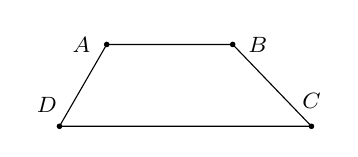
\begin{tikzpicture}[scale=.8,font=\footnotesize,line join=round,line cap=round,>=stealth]
				\path (0,0)coordinate(A)+(0:2)coordinate(B)++(-120:1.5)coordinate(D)+(0:4)coordinate(C);
				\foreach \i/\j in {A/180,B/0,C/90,D/120}
				\draw[fill=black] (\i)node[shift=(\j:.32)]{$\i$}circle(1pt);
				\draw (A)--(B)--(C)--(D)--cycle;
			\end{tikzpicture}
		}
		\noindent
		Mà $AB\parallel CD\Leftrightarrow\dfrac{-1-x}{1}=\dfrac{2-y}{2}\Leftrightarrow 2x-y=-4\Leftrightarrow 2-y=-2-2x$.\hfill(2)\\
		Thay (2) vào (1) ta được $(x+1)^2+4(x+1)^2=5\Leftrightarrow (x+1)^2=1\Leftrightarrow\hoac{&x=0&\Rightarrow y=4\\&x=-2&\Rightarrow y=0.}$\\
		\begin{itemize}
			\item Với $D(0;4)$ thì $\vec{DC}=(-1;-2)$, suy ra $\vec{DC}=-\vec{AB}$, suy ra $D(0;4)$ không thỏa mãn.
			\item Với $D(-2;0)$ thì $\vec{DC}=(1;2)$, suy ra $\vec{DC}=\vec{AB}$, suy ra $D(-2;0)$ thỏa mãn.
		\end{itemize}
		Tọa độ điểm thỏa mãn là $(-2;0)$. Vậy hoành độ của điểm $D$ là $-2$.	}
\end{ex}

\TL
\begin{ex}%[Mức độ H]%[BG - 10 New - 4in1,Phú Thạch]%[0H4H2-2]
	Cho $\triangle A B C$ có $BC=7$, $AC=8$, $AB=6$. Tính diện tích của $\triangle ABC$ (làm tròn kết quả đến hàng phần chục).
	% \shortans{$20{,}3$}
	\loigiai{
		Áp dụng công thức Heron với $p=\dfrac{a+b+c}{2}=\dfrac{21}{2}$.\\
		Ta có \[S=\sqrt{p\left(p-a\right)\left(p-b\right)\left(p-c\right)}=\sqrt{\dfrac{21}{2}\left(\dfrac{21}{2}-7\right)\left(\dfrac{21}{2}-8\right)\left(\dfrac{21}{2}-6\right)}=\dfrac{21\sqrt{15}}{4}\approx 20{,}3.\]
	}
\end{ex}
\begin{ex}
	Tìm số hạng chứa $y^2$ trong khai triển nhị thức Newton $(2x+3y)^4$.
	\loigiai{
		\begin{align*}
			(2x+3y)^4&=\mathrm{C}_4^0(2x)^4(3y)^0+\mathrm{C}_4^1(2x)^3(3y)^1+\mathrm{C}_4^2(2x)^2(3y)^2+\mathrm{C}_4^3(2x)^1(3y)^3+\mathrm{C}_4^4(2x)^0(3y)^4\\
			&=16x^4+96x^3y+216x^2y^2+216xy^3+81y^4.
		\end{align*}
		Vậy số hạng chứa $y^2$ trong khai triển là $216x^2y^2$.
	}
\end{ex}

\begin{ex}%[0D8V2-4]
	Một nhóm $9$ người gồm ba người đàn ông, bốn phụ nữ và hai đứa trẻ đi xem phim. Hỏi có bao nhiêu cách xếp họ ngồi trên một hàng ghế sao cho mỗi đứa trẻ ngồi giữa hai người phụ nữ và không có hai người đàn ông nào cạnh nhau?
	% \shortans[oly]{864}
	\loigiai{
		Số cách xếp $4$ người phụ nữ là $4! =24$.\\
		Có $3$ vị trí giữa $4$ người phụ nữ để xếp $2$ đứa trẻ. Do đó có $\mathrm{A}_3^2=6$ cách xếp $2$ đứa trẻ.\\
		$3$ vị trí còn lại cho $3$ người đàn ông là đầu hàng ghế, cuối  hàng ghế và vị trí còn trống giữa $3$ người phụ nữ. Do đó có $3!=6$ cách xếp $3$ người đàn ông.\\
		Vậy có $24\cdot 6\cdot 6=864$ cách sắp xếp $9$ người thỏa mãn yêu cầu bài toán.
	}
\end{ex}
\begin{ex}%[0H5C2-6]
	Cho ba lực $\vv{F_1}$, $\vv{F_2}$, $\vv{F_3}$ cùng tác động vào một vật tại điểm $M$ và vật đứng yên. Cho biết cường độ của $\vv{F_1}$, $\vv{F_2}$ đều bằng $70N$ và $\left(\vv{F_1},\vv{F_2}\right)=60^\circ$. Cường độ của lực $\vv{F_3}$ bằng $a\sqrt{b}$. Khi đó $a+b$ có giá trị là bao nhiêu?
	\loigiai{
		\begin{center}
			\begin{tikzpicture}[scale=0.3, font=\footnotesize,line join=round, line cap=round,>=stealth]
				\path (10,5)coordinate[label=below:$M$](M) (21,5)coordinate[label=below right:$C$](C) (-1,1)coordinate[label=below left:$B$](B) (-1,9)coordinate[label=above left:$A$](A) (-11,5)coordinate[label=left:$D$](D);
				\coordinate[label=above right:$\overrightarrow{F_1}$] (F1) at ($(M)!0.8!(A)$);
				\coordinate[label=below right:$\overrightarrow{F_2}$] (F2) at ($(M)!0.85!(B)$);
				\coordinate[label=above:$\overrightarrow{F_1}+\overrightarrow{F_2}$] (F4) at ($(M)!0.55!(D)$);
				\coordinate[label=above:$\overrightarrow{F_3}$] (F2) at ($(M)!0.5!(C)$);
				\draw[-stealth] (M)--(B);
				\draw[-stealth] (M)--(C);
				\draw[-stealth] (M)--(A);
				\draw[-stealth] (M)--(D);
				\draw[dashed] (A)--(D)--(B);
				\tkzDrawPoints[fill=black](M)
			\end{tikzpicture}
		\end{center}
		Ta có $\overrightarrow{F_1}+\overrightarrow{F_2}=\overrightarrow{MA}+\overrightarrow{MB}=\overrightarrow{MD}$ (Với $D$ là điểm sao cho $AMBD$ là hình bình hành).\\
		Ta có $MA=\left|\overrightarrow{MA}\right|=\left|\overrightarrow{F_1}\right|=70$ N; $MB=\left|\overrightarrow{MB}\right|=\left|\overrightarrow{F_2}\right|=70$ N.\\
		Do $\widehat{AMB}=60^\circ$ nên $\triangle AMB$ là tam giác đều. Khi đó $MD=2\cdot\dfrac{70\sqrt{3}}{2}=70\sqrt{3}$ (N).\\
		Do vật đứng yên nên cường độ lực tác dụng lên vật bằng $0$ hay $\overrightarrow{F_1}+\overrightarrow{F_2}+\overrightarrow{F_3}=\overrightarrow{0}$.\\
		Suy ra $\overrightarrow{F_3}=-\left(\overrightarrow{F_1}+\overrightarrow{F_2}\right)\Rightarrow \left|\overrightarrow{F_3}\right| =\left|-\left(\overrightarrow{F_1}+\overrightarrow{F_2}\right)\right|=\left|\overrightarrow{DM}\right|=MD=70\sqrt{3}$.\\
		Vậy cường độ của $\overrightarrow{F_3}$ là $70\sqrt{3}$.\\
		Từ đó suy ra $a=70$, $b=3$. Khi đó $a+b=70+3=73$.
	}

\end{ex}

\begin{ex}%[0H9H1-6]
	Một chiếc xe khởi hành từ vị trí $A(1;2)$ và di chuyển với vận tốc không đổi được biểu diễn bởi véc-tơ $\overrightarrow{v}=(2;3)$. Xe sau khi di chuyển trong $2$ giờ đến vị trí $B(x;y)$. Sau đó xe tiếp tục di chuyển theo hướng Nam với vận tốc có độ lớn bằng $4$ đến vị trí $C$. Xác định toạ độ của $C$.
	% \shortans{$18$}
	\loigiai{
		Do xe khởi hành từ $A$ di chuyển với vận tốc được biểu thị bởi véc-tơ $\overrightarrow{v}=(2;3)$ nên cứ sau mỗi giờ, xe di chuyển được một quãng đường bằng $\left| \overrightarrow{v} \right|$.\\
		Vậy sau $2$ giờ xe du chuyển tới $B$, ta được $\overrightarrow{AB}=2\overrightarrow{v}$.
		Ta có \[\overrightarrow{AB}=2\overrightarrow{v} \Leftrightarrow (x-1;y-2)=2(2;3) \Leftrightarrow \heva{&x-1=4\\&y-2=6} \Leftrightarrow \heva{&x=5\\&y=8.}\]
		Vậy sau $2$ giờ xe ở vị trí (trên mặt phẳng tọa độ) là $B(5;8)$. Do đó toạ độ vị trí $C$ là $(5;4)$
	}
\end{ex}
\Closesolutionfile{ans}

